\label{sec:overview}

\begin{figure*}[!t]
\centering
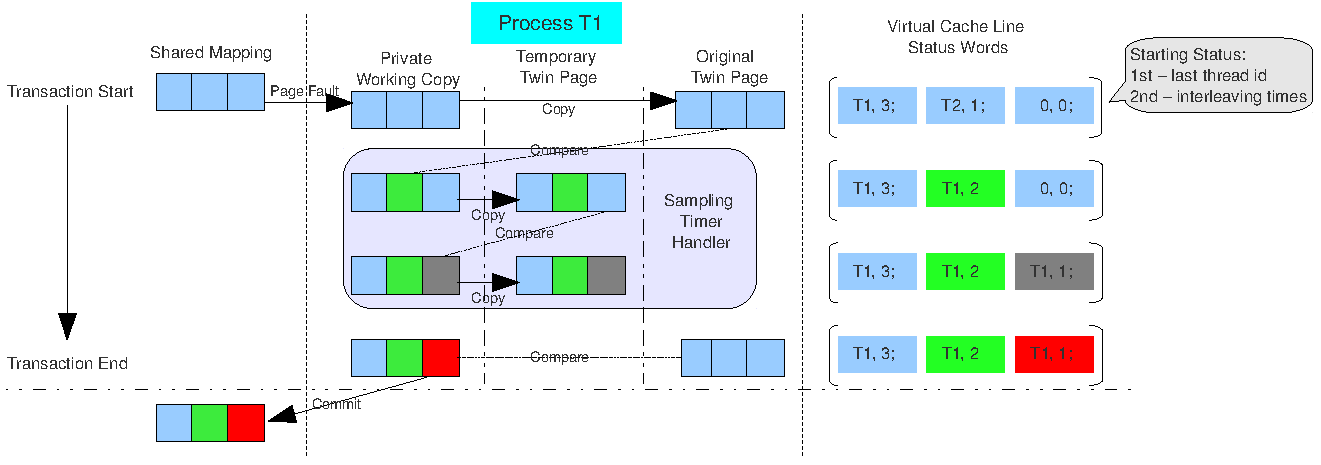
\includegraphics[height=2.3in]{figure/overview.pdf}
\caption{
Overview about the execution of Sheriff(Section~\ref{simulation:thread}). 
Sheriff simuates threads using processes(Section~\ref{sec:simulation}). 
Each process works on its private copy  
and commits modifications of current process to shared mapping in the end of transaction(Section~\ref{simulation:endtran})
relying on ``twin page mechanism''(Section~\ref{overview-twinpage}) to get difference. 
To get interleaving writes for detecting false sharing, 
we introduce virtual cache line status words (Section~\ref{detection:invalidation}) 
and sampling mechanism(Section~\ref{detection:sampling}). 
No need for sampling mechanism and status words if only for a runtime system.
\label{fig:overview}}
\end{figure*}

Unlike previous tools, Sheriff is designed based on a completely different approach.
Sheriff doesn't rely on the hardware performance counter or binary instrumentation to find out false sharing problems. 
Alternatively, Sheriff tries to design a runtime system to simulate the running of multi-threaded program and 
monitor memory writes on different virtual cache lines from different threads.
%After the finding of cache lines with numerous interleaving writes,
Sheriff can precisely locate those objects or some fields inside objects causing serious performance problem. 

\subsection{Observations and Targets}
\label{overview:target}
There are two different types of false sharing problems according to 
the definitions of Hyde and Fleisch~\cite{falseshare:Analysis}. 
One is called as ``false sharing'' when multiple structurally unrelated objects 
are located in the same cache line. 
Another is called as ``pseduo sharing'' when multiple processors 
are accessing different fields of the same object.
Sheriff aims to find these two kinds of false sharing problems. 

Note that false sharing not always cause the performance problem. 
Whether one false sharing can cause performance problems depends on memory accessing pattern. 
We observe that false sharing can cause significant performance problems 
only when there are a lot of \textbf{interleaving} memory writes from different threads. 
Based on this observeration, Sheriff is trying to capture interleaving writes from different threads and 
report only those possible false sharing causing performance problem.
%%%%%%%%%%%%%%%%%%%%%%%%%%%%%%%%%%%%%%%%%%%%
%%%%% For global objects, Sheriff can tell the name of global objects which cause the false sharing problems.
%%%%% For heap objects, Sheriff can tell the callsite of malloc, thus programmer can 
%%%% refer to actual source code to find out which object caused the problems.
%%%%%%%%%%%%%%%%%%%%%%%%%%%%%%%%%%%%%%%%%%%%5
%Sheriff won't intend to find instructions that cause false sharing problems. Since multiple 
%instructions located in different functions can cause the same false sharing problem, but without the enough times 
%to capture the attention of programmer.
\begin{comment} 
There are two ways to tell false sharing problems. One is to tell users about the placement to 
touch those false sharing objects. Now PTU can point out functions to access specified addresses, without 
the name of false sharing objects, users should still try to figure out false sharing objects
in the whole function then they can decide how to fix the problem. 
Another is to tell users about false sharing objects, then user can find how false sharing happens.  
\end{comment} 
In order to reduce the manual overhead to locate the root of false sharing problems, Sheriff tries to indentify 
false sharing objects directly. 

Since Sheriff tries to replace those standard pthreads library (including memory allocator) 
in order to avoid the false positive problems 
caused by heap objects, Sheriff can not be used to detect those false sharing problems 
caused by memory allocator. 
We believe that is also reasonable since mordern memory allocator are trying to 
avoid false sharing problems as 
much as possible~\cite{BergerMcKinleyBlumofeWilson:ASPLOS2000}. 
%Section~\ref{effect-application} examplify the easiness to find the root of false sharing problem by using Sheriff.
\subsection{Assumptions}
\label{overview:assumption}
Sheriff has a basic assumption about those evaluating programs 
in order to simulate them correctly using multiprocess mechanism.
Those evaluated program are expected to no synchronization errors, 
such as deadlock, race condition or atomicity violations. 
We believe that this assumption is reasonable. 
If there are some synchronization problems inside, applications running using Sheriff
may have a higher probability to run uncorrectly, which can prevent Sheriff to find out all false sharing problems.

\subsection{Process as Threads}
One basic mechanism of Sheriff is to treat threads as processes, which is used firstly by Grace~\cite{grace}.
%But Sheriff discards the sequential semantics of Grace, which Grace tends to use that to avoid concurrency errors. 
%Also, Sheriff discards the limit of Grace (no synchronization inside) and try to provide a framework
%which can work on general multi-threaded programs. 
Process has its own address space and signal handler table, provides strong isolation between different threads, 
which makes it perfect for Sheriff
to monitor memory accesses from different threads.
More importantly, we can utilize process to eleminate false sharing inside, no need
to let other threads to know results if no explicit synchronization.

There is a natural concern about the performance to use process instead of threads.
Although the overhead to create and exit one process is       
much more than that for one thread, we don't need pay too much overhead here since  
thread's creation and exit won't happen frequently and normal execuation of Sheriff 
can be almost the same speed as that of processes.

Section~\ref{sec:simulation} gives more details about how to simulate threads using process.
\subsection{Twin Page Mechanism}
\label{overview-twinpage}
Sheriff can capture those pages modified by one process 
when one process are trying to write on those pages protected as read-only mode.
But it is clear that page granularity is too coarse to locate cache false sharing problems.  
To avoid this problem, Sheriff are trying to use twin page mechanism to find the modifications on words. 
Twin page mechanism was first used in Munin~\cite{dsm:treadmarks} to 
capture modifications on a page in distributed share memory system.

The mechanism 
can be seen in Fig.~\ref{fig:overview}. 
Before one working page is modified, a ``twin page'' is created which is indentical
to the working page which are going to be modified. The twin page is keeping intact when the working
page are modfied. 
Later, the twin page and the working page can be compared byte by byte
later in order to capture those modifications made on the working page.
\begin{comment}
In the beginning of one synchronization phase, all pages are protected. 
At the first write on one protected page,
a page protection violation occurs. 
Operating system should send a signal handler to current process causing protection violation, 
then in the signal handler Sheriff can makes a copy of current page (creation of a twin page) 
and removes the protection on this page so that future 
writesi (in the same phase) on this page can run at a full speed. 
The twin page and the working copy of current process can be compared word by word
later to capture those writes on this page in one phase.
\end{comment}
More details about using the ``twin page mechanism'' can be seen in Section~\ref{sec:falseshare}.
%In this meaning, we are trying to introduce the "twin" mechanism used in DSM system in a general multithreaded
%program by leveraging constructively the process mechanism in the same time. 
